% !TeX program = pdfLaTeX
\documentclass[12pt]{article}
\usepackage{amsmath}
\usepackage{graphicx,psfrag,epsf}
\usepackage{enumerate}
\usepackage{natbib}
\usepackage{textcomp}
\usepackage[hyphens]{url} % not crucial - just used below for the URL
\usepackage{hyperref}
\providecommand{\tightlist}{%
  \setlength{\itemsep}{0pt}\setlength{\parskip}{0pt}}

%\pdfminorversion=4
% NOTE: To produce blinded version, replace "0" with "1" below.
\newcommand{\blind}{0}

% DON'T change margins - should be 1 inch all around.
\addtolength{\oddsidemargin}{-.5in}%
\addtolength{\evensidemargin}{-.5in}%
\addtolength{\textwidth}{1in}%
\addtolength{\textheight}{1.3in}%
\addtolength{\topmargin}{-.8in}%

%% load any required packages here




\usepackage{setspace}\doublespacing

\begin{document}


\def\spacingset#1{\renewcommand{\baselinestretch}%
{#1}\small\normalsize} \spacingset{1}


%%%%%%%%%%%%%%%%%%%%%%%%%%%%%%%%%%%%%%%%%%%%%%%%%%%%%%%%%%%%%%%%%%%%%%%%%%%%%%

\if0\blind
{
  \title{\bf Kaggle-in-class Data Challenges Can Boost Student Learning}

  \author{
        Julia Polak \\
    Department of Statistics, University of Melbourne\\
     and \\     Dianne Cook \\
    Department of Econometrics and Business Statistics, Monash University\\
      }
  \maketitle
} \fi

\if1\blind
{
  \bigskip
  \bigskip
  \bigskip
  \begin{center}
    {\LARGE\bf Kaggle-in-class Data Challenges Can Boost Student Learning}
  \end{center}
  \medskip
} \fi

\bigskip
\begin{abstract}
Kaggle is a data modeling competition service, where participants
compete to build a model with lower predictive error than other
participants. Several years ago they released a simplified service that
is ideal for instructors to run competitions in a classroom setting.
This paper describes the results of an experiment to determine if
participating in a predictive modeling competition enhances learning.
The evidence suggests it does. In addition, students were surveyed to
examine if the competition improved engagement and interest in the
class.
\end{abstract}

\noindent%
{\it Keywords:} instructional technology, statistical modeling, data science, statistics education, data mining
\vfill

\newpage
\spacingset{1.45} % DON'T change the spacing!

\providecommand{\tightlist}{%
    \setlength{\itemsep}{0pt}\setlength{\parskip}{0pt}}







\section{Introduction}\label{introduction}

Kaggle \citep{kaggle} is a platform for predictive modelling and
analytics competitions where participants compete to produce the best
predictive model for a given data set. It is well-known for its
competitions (e.g. \citet{darkmatter}), some of which come with rich
monetary prizes (e.g. \citet{heritage}). There are also learning
competitions \citep{kagglelearn}, designed to help novices hone their
data mining skills. Winners are typically expected to share their code,
and occasionally newly emerged algorithms are introduced to the broad
community, for example, deep neural networks \citep{HintonDahi12} and
XGBoost \citep{ChenXGBoost}.

In 2015, Kaggle InClass was introduced, as a self-service platform to
conduct competitions. These competitions can be private, limited to
members of a university course, and are easy to setup. This is an
opportunity for educators to provide a vehicle for students to
objectively test their learning of predictive modelling. As a
competition, with an independent clear performance metric, along with a
dynamic leader board, students can see how their model predictions
compare with the models produced by other students. Being able to make
multiple submissions over a several week time frame, enables them to try
out approaches to improve their models. This paper examines the
educational benefits of conducting predictive modeling competitions in
class on performance, engagement and interest.

In the past few years, the educational community started to collect
positive evidence on including competitions in the classroom. None of
these were data analysis competitions. \citet{VanNuland15} ran a
competition assessing anatomical knowledge, as part of an undergraduate
anatomy course. \citet{Calnon12} discusses robotics competitions as part
of computer science education. \citet{Canada15} discusses the
participation of students in externally run artificial intelligence
competitions. All of these studies found significant improvement in
student exam marks accredited to participation in competition.

Classroom competition is an example of active learning, which has been
shown to be pedagogically beneficial. \citet{Prince04} surveyed the
literature and found that all forms of active learning have positive
effect on the learning experience and student achievement. The magnitude
of the effect of different approaches, though, varies. What's more,
\citet{Freeman14} examined 158 studies published in about 50 STEM
educational journals. The authors found that student exam scores
increased by almost half a standard deviation through active learning.
Moreover, students in classes with traditional lecturing were 1.5 times
more likely to fail than their peers in classes with active learning.

A competition, like any other active learning method, that used for
assessment, has its advantages and disadvantages. It brings the `game'
feeling, increases the interest level among students and motivates for
higher performance (\citet{Shindler09}, p 105). However, it may have
negative influence if constructed poorly. Among the negative influences
are increased stress and anxiety, induced by fearing a low ranking,
failure or technology barriers. In addition, students may invest a
disproportionate amount of time and effort into competition. Despite
some received criticism, a properly set competition can benefit the
students greatly. The competition should be relatively short in duration
to avoid consuming undue energy. Students should be clear about the
rules and the goal. They should be properly rewarded and most important,
feel that they have reasonable chance to win or achieve high mark
\citep{Shindler09}.

\citet{Shelley08} raised the need for more quantitative and statistical
analysis of evidence in science education. This paper contributes to
this call by offering statistical analysis of the effects on learning of
classroom data competitions.

\section{Experimental setup}\label{experimental-setup}

\subsection{Data collection}\label{data-collection}

The experiment was conducted during Semester 2 2017. Data was collected
during two classes, one at the University of Melbourne (Computational
statistics and data mining, MAST90083, denoted as CSDM), and one at
Monash University (Statistical thinking, ETC2420/5242, denoted as ST).

\subsection{Competition data}\label{competition-data}

Two data sets were compiled for the kaggle challenges: Melbourne
property auction prices and spam classification. The Melbourne auction
price data was collected by extracting information from real estate
auction reports (pdf) collected between Feb 2, 2013 and Dec 17, 2016.
The spam classification data was compiled by graduate students at Iowa
State University as part of a data mining class in 2009. Data was
compiled by monitoring and extracting information from their emails by
class members, over a period of a week, and manually tagging them as
spam or ham.

Both data sets were split into training and test sets, for the kaggle
challenge. Students had access to the true response variable only for
the training data. For the Melbourne housing data, students were
expected to predict price based on the property characteristics. For the
spam data, students were expected to build a classifier to predict
whether the email as spam or not.

Both data sets are challenging for prediction, with relatively high
error rates.

The training and the testing data sets of the Melbourne auction price
data were similar but not identical across the two institutions. Some of
the variables in the data set were simulated, e.g.~property land size
and house size. The simulated data was generated slightly differently
for different institutions. This was done deliberately to prevent
students passing answers from one institution to another.

\subsection{Participants}\label{participants}

Computational Statistics and Data Mining (CSDM) is designed for
postgraduate level students with math, statistics, information
technology or actuarial backgrounds. It covers modelling both continuous
(regression) and categorical (classification) response variables. The 63
students were randomized into one of two kaggle competitions, one
focused on regression (R) and the other classification (C). (One of the
63 students elected not to take part in the competition, and another
student didn't sit the exam, producing a final sample size of 61.) This
setup mimics randomized control trials, which is the gold standard, in
experiment design (\citet{Shelley09CH1}, ch.~1). Students built
prediction models and made submissions individually for 16 days, and
then were allowed to form groups to compete for another 7 days.

The reason for this strategy was first to motivate each of the students
to think about modelling and be actively engaged in the competitions
through individual submission. The lecturer allowed participants to
create groups towards the end of the competition to illustrate the
advantages of group work and ensemble models. Another reason for this
approach was the university policy, requiring a strategy to assign
students individually in group assignments. When the team members
develop the model together, it is quite difficult to accurately assess
the individual contribution of each student. The individual submissions
helped to encourage each student to engage in the modelling process. In
addition, it helped to assess the individual component of the final
score for the competition.

Table 1 compares the summary statistics for the two groups. We examine
the percentage correct overall on the final exam for the different
groups and the scores the students received for the second assignment.
The second assignment examined students knowledge about computational
methods, unrelated to the classification and regression methods. The two
groups statistics are similar.

\begin{table}[h]
\begin{center}
\begin{tabular}{l l | r | r | r r r r r}\hline
Score & Comp. group & N & Mean (SD)   & Min  &  Q1 & Median  &  Q3  & Max \\\hline
Exam   & Regression      & 30 &  66.9 (14.1)  &   36.0 &  57.5 &   69.2 &  77.5 &   88.5\\
       & Classification & 31 &  62.1 (17.2)  &   20.0  & 52.2  &  68.0   &  75.2 &  85.5\\\hline

2$^{nd}$ assignment & Regression      &    30  & 8.2 (2.2)  &  0.0  & 7.0 &  8.4   &  9.9  &   10.0 \\
                    & Classification  &    31  & 8.0 (3.0)  &  0.0  & 7.8  &  9.3   &  9.9  &   10.0 \\\hline

\end{tabular}
\caption{Computational statistics and data mining: Summary statistics of the exam score (out of 100) and the second assignment (out of 10) for the two competition groups.}
\end{center}
\label{tab:Melb_Group_Compare}
\end{table}

Statistical Thinking (ST), covers regression, but not classification,
and has a mix of undergraduate and postgraduate students. Only the 34
postgraduate (ST-PG) students were required to participate in the kaggle
competition, and competed in the regression (R) challenge. This was run
independently from the CSDM competition. The 145 undergraduate (ST-UG)
students were used as comparison for examining performance of the
postgraduate students. Although, it may be surprising at first glance,
the undergraduate students provide a reasonable comparison for the
graduate students. The class is taught to both cohorts simultaneously.
The entry requirements to the Bachelors of Commerce at Monash is high,
and these students have strong mathematics backgrounds. In the years
prior to this experiment, the undergraduate scores on the final exam are
indistinguishable from those of the graduate students. The competition
ran for one month. Students formed their own teams of 2-4 members to
compete.

Table 2 shows the summary statistics of the exam scores for the 34
postgraduate (ST-PG) students and for the 145 undergraduate (ST-UG)
students. The mean and the median scores of postgraduate students are a
bit lower than the corresponding scores of undergraduate students.
However, the interquartile range is similar. Interestingly, the highest
exam score was received by an undergraduate student.

\begin{table}[h]
\begin{center}
\begin{tabular}{l l | r | r | r r r r r}\hline
Score & Competition group & N & Mean (SD)   & Min  &  Q1 & Median  &  Q3  & Max \\\hline
Exam   & ST-PG      & 34  & 61.8 (12.2)  &  35.0 & 57.2  &   61.0  & 72.2  & 81.5 \\
       & ST-UG         & 145 & 63.0 (15.4)  &   0.0 & 56.0  &   64.0  & 73.0   & 90.0\\\hline
\end{tabular}
\caption{Statistical thinking: Summary statistics of the exam score (out of 100) for the two groups.}
\end{center}
\label{tab:Melb_Group_Compare}
\end{table}

Figure \ref{fig:Monash_quiz} displays the quiz scores taken by the
undergraduate (ST-UG) and postgraduate (ST-PG) students, as a beeswarm
plot \citep{beeswarm}. The distribution of quiz scores are similar,
except that undergraduates tend to have a longer lower tail.

\begin{figure}
\centering
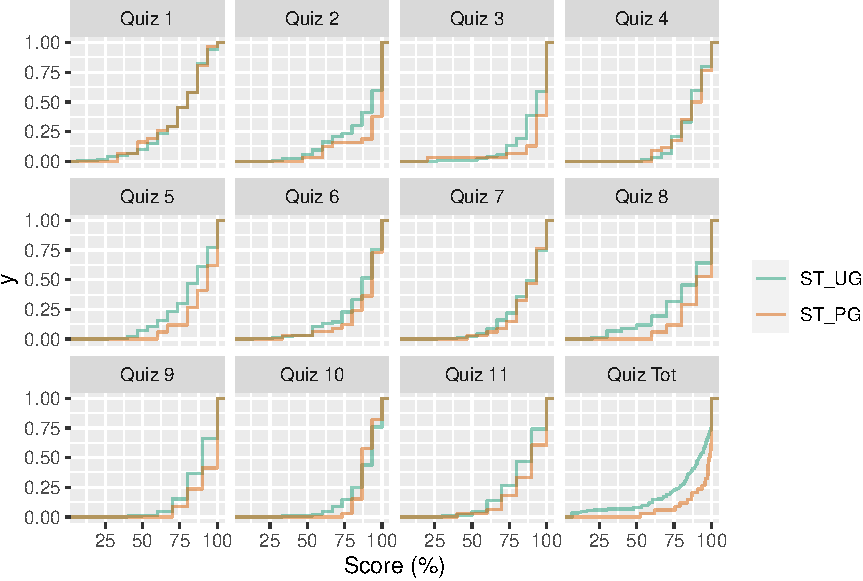
\includegraphics{paper-kaggle_files/figure-latex/Monash_quiz-1.pdf}
\caption{\label{fig:Monash_quiz}Beeswarm plots of undergraduate (ST-UG)
and postgraduate (ST-PG) students quizzes during the semester. The
scores are very similar, although undergraduates have a longer lower
tail.}
\end{figure}

\section{Methodology}\label{methodology}

\subsection{Performance}\label{performance}

Better performance is equated to better understanding of the material,
as measured in the final exam. CSDM and ST included questions, with
several parts, on the final exam related to kaggle challenges. These
questions were identified prior to data analysis.

For all questions in the exam, difficulty and discrimination scores were
computed, using the mean and standard deviations. Of the questions
pre-identified as being relevant to the data challenges, only the parts
that corresponded to high level of difficulty and high discrimination
were included in the comparison of performance.

Scores for the relevant questions were summed, and converted into
percentage of the possible score. The total exam score was converted to
a percentage. One can expect, that on average, student's success rate
for each question will be about the same as the success rate in the
total exam. Understanding one topic better than another will result in
higher success rate for questions asking about the better understood
topic compared to the scores for other topics. For example, we would
expect from a student with a 70\% exam mark to get 70\% marks on each of
the questions in the exam, if she has similar knowledge level on all the
exam topics. If in some topic, say regression, the student has better
knowledge, she will perform better on the regression questions. Her
success rate on regression question will be higher than 70\%.
Consequently, her performance on some other questions should be below
70\% which is associated with lesser understanding of these topics.

Therefore, performance for each student was computed as the ratio of
these two numbers, percentage success in the regression (classification)
questions and percentage success in the total exam. A value of 1 would
indicate that the student's performance on that set of questions was
consistent with their overall exam performance, greater than 1 that they
performed better than expected, and lower than 1 meant less than
expected on that topic.

Using only the percentage of successes for each set of questions,
instead of the proposed ratio, will not differentiate between a better
performance and just a better student. Especially in the case of ST that
have a mixed population of master and undergraduate student.

The distribution of the performance scores by group is shown as a
boxplot. Focus is on the difference in median between the groups.
Permutation tests were conducted to examine difference in median scores
for students participating or not in a competition.

\subsection{Engagement}\label{engagement}

The students were allowed to submit at most one prediction per day,
while the competitions were open. The frequency of submissions, and the
accuracy (or error) of their predictions, made by individual students,
is recorded as a part of the kaggle system. To examine whether
engagement improved performance, scores on the questions related to the
competition normalised by total exam score (as computed in the
performance section) is examined in relation to frequency of submissions
during the competition. In addition, performance in the competition as
measured by accuracy or error, is also examined in relation to the
number of submissions. Scatterplots, correlation and linear models are
used to examine the associations.

\subsection{Interest}\label{interest}

Students in CSDM and ST-PG were invited to give feedback about the
course, in particular about the data competitions, before the final
exam. This information was voluntary, and students who completed the
questionnaire were rewarded with a coupon for a free coffee. The data
from this survey was viewed by the researchers after all course grades
had been reported. To reduce potential bias in students replies, we
emphasize this point as part of the instruction at the beginning of the
survey.

\section{Results}\label{results}

\subsection{Performance}\label{performance-1}

Figure \ref{fig:MAST90083} shows the data collected in CSDM. Performance
is plotted against type of question, separately for the competition they
completed. The difference in median scores indicates performance
improvement. Students who completed the classification competition
(left) performed relatively better on the classification questions than
the regression questions in the final exam. Conversely, students who
participated in the regression competition performed relatively better
on the regression questions.

\begin{figure}
\centering
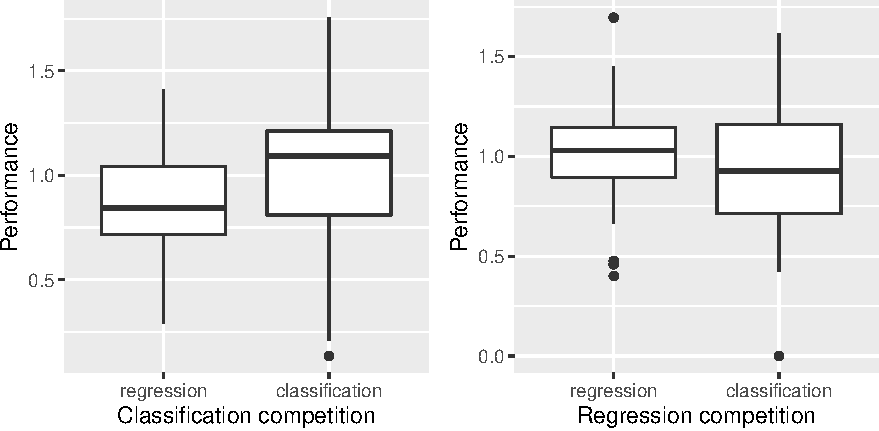
\includegraphics{paper-kaggle_files/figure-latex/Melb-1.pdf}
\caption{\label{fig:MAST90083} Boxplots of performance on regression and
classification questions in the final exam, by type of data competition
completed in CSDM. Students generally performed better on the questions
corresponding to the competition they participated in.}
\end{figure}

\begin{table}[h]
\begin{center}
\begin{tabular}{|l|r|r|}\hline
Question Set & Median difference & Permutation $p$-value \\\hline
Classification & 0.250 & 0.033\\
Regression & 0.104 & 0.000\\\hline
\end{tabular}
\caption{Comparison of median difference in performance by competition group, for CSDM students, using permutation tests. Both sets of medians are significantly different, indicating improved scores for questions on the topic related to the Kaggle competition.}
\end{center}
\label{tab:Melb_Perm}
\end{table}

Table 3 shows the results of permutation testing of median difference
between the groups. Generally the results support the competition
improved performance. Students who participated in the kaggle challenge
for classification scored higher than those that did the regression
competition, on the classification problem. Using a permutation test,
this corresponds to a significant difference in medians. Similarly the
results show that students who did the regression challenge, performed
better on these exam questions.

Figure \ref{fig:ETC5242} shows the results for ST students. The boxplots
suggest that the students who participated in the challenge performed
relatively better than those that didn't on the regression question than
expected given their total exam performance.

Only the post-graduate students participated in the regression
competition, as their additional assessment requirement. Scores for the
question on regression (Q7a,b,c) in the final exam were compared with
the total exam score (RE). On these question parts, a, b, c, over all
the students all three were in the top 10 of difficulty, with students
scoring less than 70\%, on average. Parts b, c were in the top 10 for
discrimination, and part a was at rank 13.

\begin{figure}
\centering
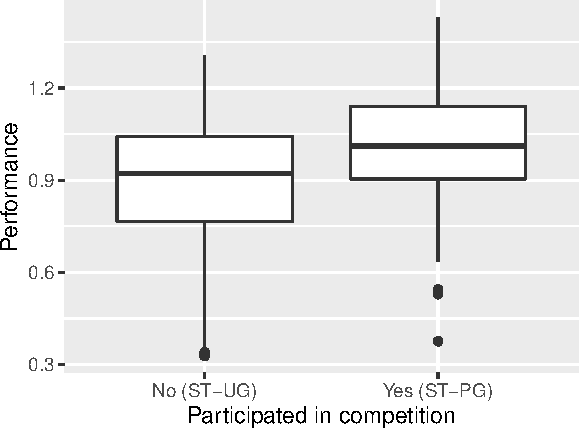
\includegraphics{paper-kaggle_files/figure-latex/ETC5242-1.pdf}
\caption{\label{fig:ETC5242} Performance for regression question
relative to total exam score for students who did and didn't do the
regression data competition in Statistical thinking.}
\end{figure}

Based on the median, the students who participated in the kaggle
challenge scored 0.09 higher than those that didn't, a median of 1.01 in
comparison to 0.92. Using a permutation test, this corresponds to a
significant difference in medians, with \(p\)-value of 0.024.

\begin{figure}
\centering
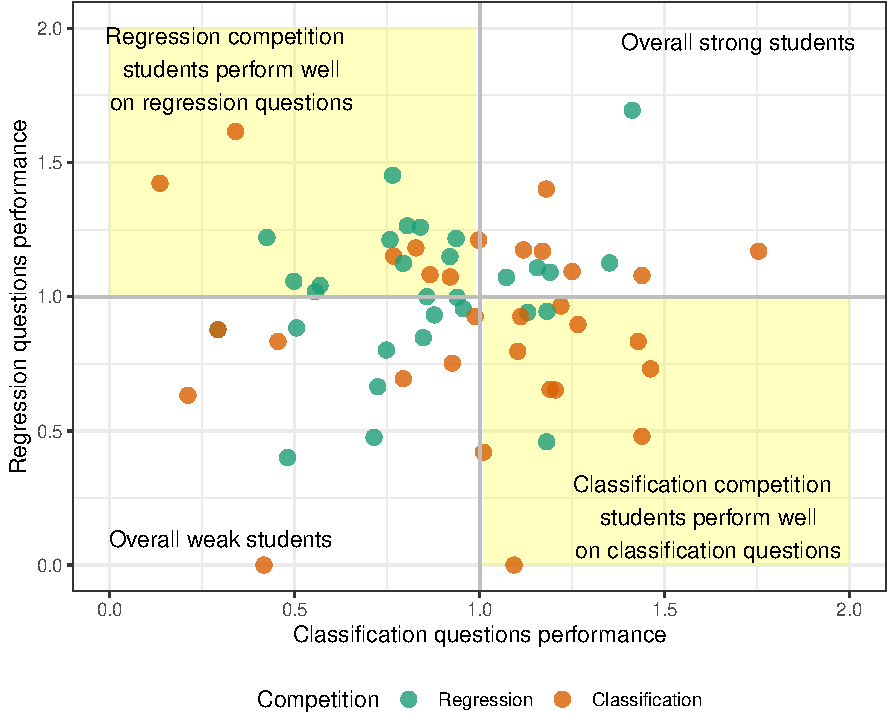
\includegraphics{paper-kaggle_files/figure-latex/crossperformances-1.pdf}
\caption{\label{fig:crossperformances} Students performance in
classification and regression questions by competition type.}
\end{figure}

Figure \ref{fig:crossperformances} presents students' scores for
classification and regression questions. A score over 1 is considered as
outperform (relative to the expectation). Quarters one and three include
students that underperform or outperform on both types of questions,
respectively. In both cases the number of students that participated in
the classification competition is very close to the number of students
that participated in the regression competition (excluding a few
regression students on the border of score 1). Students in quarters two
and four outperform on one type of questions but not on the other type.
We can see that more regression students outperform on regression
questions than classification students (12 vs. 7). Similarly,
classification students do better on classification questions (11 vs.
3). This is another evidence towards positive influence of the data
competition on student's performances.

\subsection{Engagement}\label{engagement-1}

The number of submissions that a student made, may be an indicator of
performance on the exam questions related to the competition. A student
who is more engaged in the competition may learn more about the
material, and consequently perform better on the exam. Figure
\ref{fig:numsubmition} (top row) shows performance on the classification
and regression questions, respectively, against their frequency of
prediction submissions for the three student groups (CSDM classification
and regression, ST-PG regression) competitions. The relationship is weak
in all groups, and this mirrors insignificant results from a linear
model fit to both subsets. On the other hand, the predictive accuracy
improved with the number of submissions for the regression competitions.
There appears to be some nonlinearity present in these plots, suggesting
reduced returns. That is reasonable to expect. Also, some students
strategically make very poor initial predictions, to get a baseline on
error equivalent to guessing.

The competition performance relative to number of submissions is shown
in plots (d)-(f). Each point corresponds to one student, and accuracy or
error of the best predictions submitted is used. The regression
competition seemed to engage students more than the classification
challenge. Students submitted more predictions, and their models
improved with more submissions.

\begin{figure}
\centering
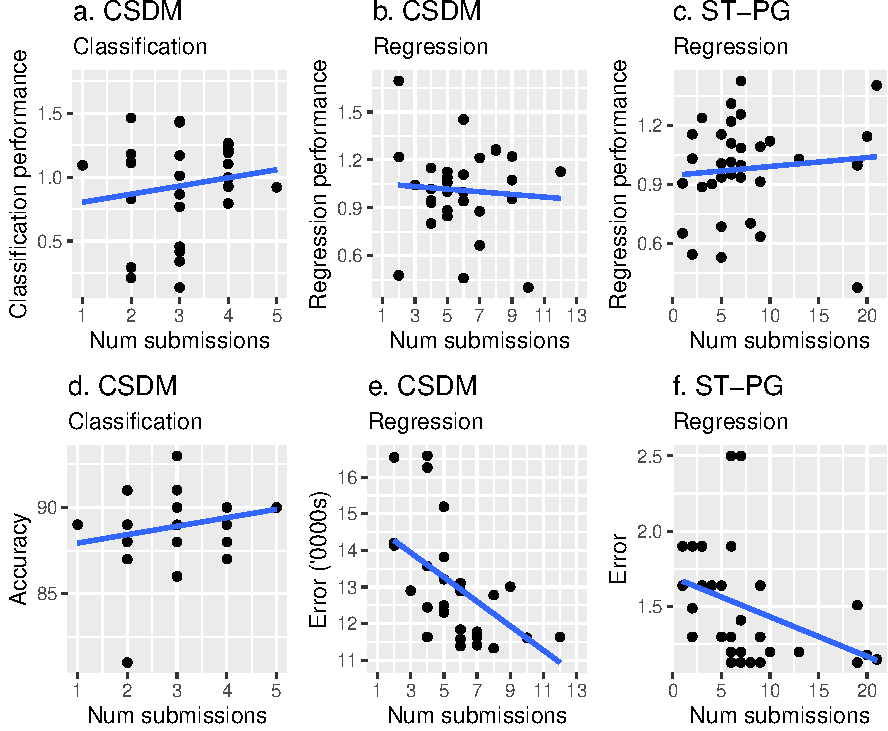
\includegraphics{paper-kaggle_files/figure-latex/numsubmition-1.pdf}
\caption{\label{fig:numsubmition} Scatterplots of the exam performance
(a-c) and competition performance (d-f) by number of prediction
submissions, for the three student groups. The relationships with exam
performance are weak. For the CSDM and ST-PG regression competitions, a
clear pattern is that predictions improved substantially with more
submissions. (House price in ST-PG were divided by 100,000, explaining
the difference in magnitude of error between two competitions.)}
\end{figure}

\subsection{Interest}\label{interest-1}

Figure \ref{fig:likert} shows the survey responses related to the kaggle
competition, for CSDM and ST-PG. The response rate for CSDM was 55\%,
with 34 of 61 students completing the survey. The response rate for
ST-PG was 50\%, 17 students out of 34 completed the survey.
Overwhelmingly, students reported that they found the competition
interesting and helpful for their learning in the course.

\begin{figure}
\centering
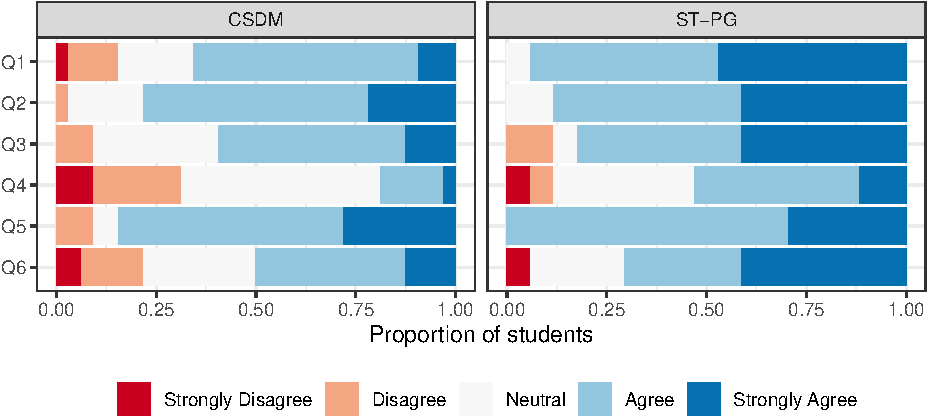
\includegraphics{paper-kaggle_files/figure-latex/likert-1.pdf}
\caption{\label{fig:likert}Summary of responses to survey of kaggle
competition participants. Overwhelmingly the response to the competition
was positive in both classes, especially the questions on enjoyment and
engagement in the class, and obtaining practical experience. (Table 4
lists the questions.)}
\end{figure}

\begin{table}[b!]
\begin{center}
\begin{tabular}{|l|p{15cm}|}\hline
Label & Question \\\hline
Q1 & I found the data competition is great fun.\\\hline
Q2 & Taking part in the data competition contributed a lot to my engagement with the subject.\\\hline
Q3 & Taking part in the data competition improved my confidence in my understanding of the covered material.\\\hline
Q4 & Taking part in the data competition improved my confidence in my success in the final exam.\\\hline
Q5 & Taking part in the data competition improved my confidence in my ability to use the acquired knowledge in practical applications.\\\hline
Q6 & I feel that the required time investment in the data competition was worthy. \\\hline
\end{tabular}
\end{center}
\caption{Questions asked in the survey of competition participants.}
\label{survey_Q}
\end{table}

After collecting the survey from the students we were told that the
questions about students engagement were positively worded. This may
have potentially led to some bias. An improved way could be to ask
directly about student's engagement, e.g. ``How would you rate your
level of engagement in this course?'' with set answer options of ``not
at all engaged'' -- up to ``extremely engaged'' with several choices in
between. Another improvement could be asking ST-UG students that didn't
take part in the competition about their level of engagement and compare
the answers with other students of ST-PG. We acknowledge that the
differences in the engagement levels may not necessarily be a result of
participation in the competition but it is still an interesting aspect.

The survey was not anonymous. However, the results became available to
the lectures only after all the grades were realised to the students.
This point was emphasized in the instructions to the students at the
beginning of the survey.

\section{Teachers' corner}\label{teachers-corner}

Creating a new competition is surprisingly easy. Information on setting
up a Kaggle InClass challenge is available on the service's web site
(\url{https://www.kaggle.com/about/inclass/overview}). There is a setup
wizard for step-by-step guidance on getting your competition underway.
We have created a short video illustrating the steps to establish a new
competition, available on the web
(\url{https://www.youtube.com/watch?v=tqbps4vq2Mc&t=32s}).

The kaggle service provides some data sets, primarily for student
self-learning. These are not suitable for use in a class challenge,
because all the data is available, and solutions are also provided. We
recommend providing your own data for the class challenge. Finding a
suitable data set for a competition can be a difficult task. The
criteria for a good data set are:

\begin{enumerate}
\def\labelenumi{\arabic{enumi}.}
\tightlist
\item
  the full set is not available to the students, to avoid plagiarism and
  use of unauthorized assistance.
\item
  the data is not too easy, or too hard, to model so that there is some
  discriminatory power in the results.
\item
  data should be relatively clean, to the point where the instructor has
  tested that a model can be fitted.
\item
  contains some challenges, that make standard off-the-shelf modeling
  less successful, like different variable types that need processing or
  transforming, some outliers, large number of variables.
\item
  if it is a classification challenge, it will work better with
  relatively balanced classes, because the overall accuracy is the
  easiest metric to use.
\end{enumerate}

The data sets used in our competitions can be shared with other
instructors by request.

Choosing the metric upon which to evaluate the model is another
decision. Our advice is to keep it simple, so you, and the students, can
understand the student scores. If you are running a regression
challenge, then the ``Root Mean Squared Error (RMSE)'' is a good choice.
If it is a classification challenge, then ``Categorization Accuracy'',
the percent of correct classifications, is reasonable.

The data needs to be split into training and testing sets. Kaggle will
then split your test set into two, a public set that is used to provide
ongoing scores to participants, and a private set, on which performance
is revealed only after the competition closes. If you have categorical
variables in the data set, you will want to make sure that all
categories are present in both training and test sets. The training set
will have both predictors and response, but the test set will have the
response variable removed. Each observation needs to be assigned an id,
because this will be needed to evaluate predictions. The solution file,
containing the id and the true response, is provided to the system for
evaluating submissions, and is kept private. A sample submission file
needs to be provided. Participants will submit their solutions in the
same format.

It is a good idea to build a basic model yourself on the training data,
and predict the test data. The performance of this model can be provided
to the participants as baseline to beat.

The competition needs to run without any intervention from the
instructor. Exception is, of course, an academic discussion motivated by
the competition between the teaching team and the students. For example,
a discussion about different models, their advantages and limitations.
The instructor can monitor students progress: the number of submissions,
student scores and even the uploaded data at any time. When the
competition ends the ``Leaderboard'' page provides a list of students
ordered by the final score. It also provides all the scores from all
past submissions (under ``Raw Data'' on ``Public Leaderboard'').

It may be recommended to limit students to one submission per day. It
encourages students to think about more efficient improvement of their
model before the next submission. It also prevents the student spending
too much time building and submitting models. Some students will become
so engaged in the competition that they might neglect their other
coursework. About halfway through the competition, students might be
allowed to form teams, to learn how averaging models can boost
performance.

In awarding course points to student effort, we typically align it to
performance. Participant ranks based on their performance on the private
part of the test data are recorded. Performance scores that are pretty
close to each other should be given the same rank, reflecting that there
may not be a significant difference between them. The best gets perhaps,
5 points, then a half a point drop until about 2.5 points, so that the
worst performing students still get 50\% for the task. Kaggle does not
allow you to download participants email addresses. All you see is their
kaggle name. Record the student names in kaggle to match with your class
records.

Along with the competition, students were expected to submit a report
that explained their modeling strategy, and what they had learned about
the data beyond the modeling. The overall score for this part of the
course was a combination of the mark for their report and their
performance in the challenge. In both courses this accounted for 10\% of
the final mark.

From an instructor perspective, its very rewarding watching the students
participate in the competition. It provides a truly objective way to
assess their ability to model in practice. Students are often motivated
to consult with the instructor about why their model is underperforming,
or what other approaches might produce better results.

\section{Discussion}\label{discussion}

This paper has described an experiment to examine the effectiveness of
data competitions on student learning, using Kaggle InClass as the
vehicle for conducting the competition. The primary finding, is that
participating in a data challenge competition, produces a statistically
significant improvement in the learning of the topic, although the
effect size is small. Secondarily, the competitions enhanced interest
and engagement in the course.

Because the experiment was conducted in the classroom setting as part of
the normal teaching of the courses, which imposed limitations on the
design. However, performance comparison was enabled in CSDM by a
randomized assignment of students to two topic groups, and in ST by
using a control group. In CDSM, the group sizes were relatively small,
approximately 30 students per group. For ST the control group was the
undergraduate students that took class. Using undergraduate students as
a control group for graduate students may be surprising. However, the
experience of teaching this subject over several years and some
statistical comparison of the two groups justifies the approach.
Undergraduate students performance in other tasks and exam questions,
not relevant to the competition, was equivalent to the postgraduate
students cohort.

\section{Future work}\label{future-work}

This work is one of a few quantitative analyses of data competition
influences on students' performance. More evidence needs to be collected
from other STEM courses to explore consistent positive influence.
Moreover, future investigation is required to understand the influence
of the different aspects of data competition implementation on the
magnitude of the performance improvement. For example, the competition
duration, availability and accessibility of additional material,
requirement of writing a final report or giving a short oral
presentation are elements worth investigating. Prior and post testing of
students might provide a better experimental design.

\section{Acknowledgments}\label{acknowledgments}

This project (title: Effect of Data Competition on Learning Experience)
has been approved by the Faculty of Science Human Ethics Advisory Group
University of AB (ID: 1749858.1 on September 4, 2017) and by CD
University Human Research Ethics Committee (ID: 9985 on August 24,
2017).

This document was produced in R \citep{R} with the package knitr
\citep{knitr}. Data cleaning was conducted using tidyr \citep{tidyr},
dplyr \citep{dplyr} and plots were made with ggplot2 \citep{ggplot2}.
The materials to reproduce the work are available at
\url{https://github.com/dicook/paper-quoll}.

\bibliographystyle{agsm}
\bibliography{bibliography.bib}

\end{document}
